\documentclass[a4paper,12pt,fleqn]{article}%fleqn pour aligner les equations à gauche
\usepackage{../../Styles/Cours}

\newcommand{\chnum}{Chapitre 1}
\newcommand{\chtitle}{Dosage de la bouillie bordelaise}
\newcommand{\dtype}{TP 3}

\begin{document}
	\maketitle
	L’objectif de cette activité expérimentale est de déterminer la concentration d’une espèce colorée à	partir d’une courbe d’étalonnage en utilisant la loi de Beer-Lambert.
	
	\begin{figure}[h!]
		\caption{La bouillie bordelaise}
		La bouillie bordelaise est un produit de traitement fongicide efficace et autorisé en agriculture biologique. Elle est largement utilisée pour le traitement des plantes, légumes ou fruitiers du jardin.\\
		Le respect des doses et de l’utilisation de ce produit est néanmoins nécessaire pour ne pas contaminer la nature.
		\begin{itemize**}
			\item \underline{Utilisation} : fongicide, algicide
			\item \underline{Composition} : eau, sulfate de cuivre et chaux.
			\item \underline{Principales plantes concernées} : vigne, fruitiers, pomme de terre, tomates.
		\end{itemize**}
	\end{figure}
	
	\begin{figure}[h!]
		\begin{minipage}{.48\linewidth}
			\caption{Utilisation de la bouillie bordelaise}
			Il s’agit d’un fongicide de couleur bleue à	base de sulfate de cuivre et de chaux. Elle est utilisée de préférence en pulvérisation et
			sert à lutter contre la plupart des formes de maladies cryptogamiques, c’est à dire les champignons et couramment utilisée contre le mildiou, la tavelure, la cloque des fruits,	les chancres ou encore la moniliose.\\
			La dose à respecter doit être comprise entre 10 et 20 g par litre d’eau et ne doit surtout pas être dépassée.
		\end{minipage}\hspace{2em}
		\begin{minipage}{.48\linewidth}
			\caption{Spectre d'absorption des ions \ce{Cu^2+} en solution}
			\centering
			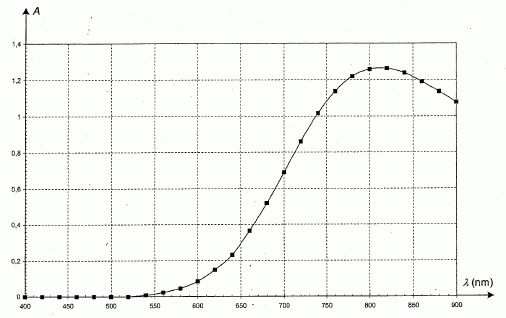
\includegraphics[width=\linewidth]{Ressources/spectreCu2.png}
		\end{minipage}
	\end{figure}
	
	\begin{figure}[h!]
		\caption{Principe du dosage}
		Pour doser par spectrophotométrie une solution de sulfate de cuivre (\ce{Cu^2+} ; \ce{SO4^2-}) de concentration en quantité de matière notée $C$, il faut disposer d'une gamme étalon.\\
		On dispose d'une solution mère $S_0$ de concentration connue égale à \SI{1,0}{mL} à partir de laquelle sont préparées 5 solutions filles notées $S_1$, $S_2$, $S_3$, $S_4$ et $S_5$.\\
		Après avoir mesuré à l'aide d'un spectrophotomètre l'absorbance de ces solutions pour une longueur d'onde idéalement choisie, on trace le graphe $A=f(C)$ et on en déduit, à partir de la droite moyenne, la concentration de la solution inconnue par lecture graphique.
	\end{figure}
	
	\begin{figure}[h!]
		\caption{Préparation des solutions filles}
		On dispose de fioles, de pipettes jaugées et graduées de différents volumes. Chaque \textbf{\underline{expliquera}} la préparation d'une solution fille. Déterminer la fiole et la pipette à utiliser pour préparer chaque solution.
		\begin{center}
			\begin{tabular}{|c|c|c|c|c|c|}
				\hline
				\textbf{Solution} & $S_1$ & $S_2$ & $S_3$ & $S_4$ & $S_5$\\
				\hline
				\textbf{Concentration (\unit{\mole\per\liter})} & \num{1,0E-1} & \num{2,0E-1}& \num{3,0E-1}& \num{4,0E-1}& \num{5,0E-1}\\
				\hline
				$V_0$ à prélever (\unit{mL}) & & & & & \\
				\hline
				$V_{solution}$ & \num{50,0} & \num{50,0} & \num{50,0} & \num{50,0} & \num{50,0}\\
				\hline
				Absorbance& & & & & \\
				\hline
			\end{tabular}
		\end{center}
	\end{figure}
	
	\begin{figure}[h!]
		\caption*{Rappels - Méthode de préparation par dilution}
		Prélever un volume $V_0$ de la solution mère $S_0$ à l’aide d’une \textbf{pipette jaugée }ou \textbf{graduée} et 		l’introduire dans une fiole jaugée de volume $V$.\\
		Choisir les volumes $V$ et $V_0$ tels que $F = \dfrac{C_0}{C} = \dfrac{V}{V_0}$, où $C$ est la concentration de la solution diluée à préparer et $C_0$ la concentration de la solution concentrée (\emph{$F$ est appelé le facteur de dilution}).\\
		Compléter la fiole jaugée avec de l’eau distillée jusqu’au trait de jauge puis homogénéiser la
		solution.
	\end{figure}
	
	\begin{figure}
		\caption*{Procédure et questions :}
		\begin{enumerate}
			\item Détermination de la longueur d'onde
		\end{enumerate}
		Le spectrophotomètre utilisé ne permet de mesurer l'absorbance d'une solution que pour quatre
		longueurs d'onde : \\
		\SI{470}{nm} (bleu) - \SI{528}{nm} (vert) - \SI{587}{nm} (jaune) - \SI{633}{nm} (rouge)\\
		On lui donne le nom de colorimètre.\\
		\textit{Déterminer, en justifiant, la longueur d'onde idéale pour effectuer les mesures de l'absorbance lors de ce dosage.}
		
		\begin{enumerate}[resume]
			\item Réglage du blanc
		\end{enumerate}
		\textit{Placer de l’eau distillée dans une cuve. Utiliser le bouton réglage du blanc afin que la valeur de la transmittance soit de} \SI{100}{\percent}.
		
		\begin{enumerate}[resume]
			\item Mesures
		\end{enumerate}
		\textit{Mesurer l'absorbance des 5 solutions filles.}\\
		\textit{Compléter le tableau.}
		\textit{Avec Latis Pro, tracer la courbe d’étalonnage A = f (C) puis modéliser.}
		
		\begin{enumerate}[resume]
			\item Exploitation
		\end{enumerate}
		\textit{Déterminer l'absorbance de la solution inconnue $S$ et en déduire, grâce à la droite
		d’étalonnage, sa concentration en quantité de matière $C_S$.}\\
		\textit{En déduire la concentration en masse $C_{mS}$ de la solution $S$.}\\
		\textit{Cette solution peut-elle être utilisée comme bouillie bordelaise ?}
	\end{figure}
	\textbf{Données :} $M (\ce{CuSO4, 5H2O}) = \SI{249,5}{\gram\per\mole}$
\end{document}